\documentclass[11pt,a4paper]{article}
\usepackage[margin=1in]{geometry}
\usepackage{beamerarticle}
\usepackage{kotex}
\usepackage{amsmath,amssymb,bm}
\usepackage{booktabs}
\usepackage{listings}
\usepackage{tikz}
\usetikzlibrary{arrows.meta,positioning,calc,shapes.geometric,fit,backgrounds}
\usepackage{hyperref}

\lstset{
  language=Python,
  basicstyle=\ttfamily\scriptsize,
  commentstyle=\color{green!40!black},
  keywordstyle=\color{blue!70!black},
  stringstyle=\color{orange!60!black},
  showstringspaces=false,
  columns=fullflexible,
  keepspaces=true,
  frame=single,
  breaklines=true
}

\title{Hands-On GNN Chapter 10}
\author{A7610 그래프신경망특론 / 조남언}
\date{\today}

\begin{document}
\maketitle
\tableofcontents
\begin{frame}
  \titlepage
\end{frame}

\begin{frame}{목차}
  \tableofcontents
\end{frame}

% =============================================================
\section{링크 예측 문제 개관}
% =============================================================

\begin{frame}{Link Prediction이란?}
\begin{itemize}
  \item 그래프 $G=(V,E)$에서 \textbf{관측되지 않은 엣지} $(u,v) \notin E$가 실제로 존재할 가능성을 추정
  \item 입력: 노드 집합 $V$, 현재까지 관측된 엣지 $E_{\text{obs}}$, (선택) 노드 특징 $X$
  \item 출력: 임의의 노드 쌍에 대한 연결 점수 $s(u,v) \in [0,1]$
\end{itemize}
\vspace{0.4em}
\textbf{대표 응용}
\begin{itemize}
  \item 소셜 네트워크의 친구 추천
  \item 추천 시스템(사용자-아이템 이분그래프)
  \item 단백질 상호작용 예측, 약물-표적 상호작용
  \item 지식 그래프 자동 완성
\end{itemize}
\end{frame}

\begin{frame}{전통적 휴리스틱과 학습 기반의 차이}
\small
\begin{tabular}{p{0.32\linewidth} p{0.62\linewidth}}
\toprule
\textbf{접근} & \textbf{점수 함수 $s(u,v)$} \\
\midrule
Common Neighbors & $|\Gamma(u)\cap\Gamma(v)|$ \\
Jaccard          & $|\Gamma(u)\cap\Gamma(v)| / |\Gamma(u)\cup\Gamma(v)|$ \\
Adamic--Adar     & $\sum_{w\in\Gamma(u)\cap\Gamma(v)} 1/\log|\Gamma(w)|$ \\
Katz, PageRank   & 경로 기반 / 랜덤워크 기반 \\
\midrule
GAE/VGAE         & $\sigma(\mathbf{z}_u^\top \mathbf{z}_v)$, $\mathbf{z}=\mathrm{GNN}(X,A)$ \\
SEAL             & 두 노드의 enclosing subgraph를 통째로 분류 \\
\bottomrule
\end{tabular}
\vspace{0.6em}
\begin{itemize}
  \item 휴리스틱: 도메인마다 잘 통하는 지표가 다름 (정해진 가정 위에서만 작동)
  \item GNN 기반: \textbf{데이터로부터} 적절한 표현/점수 함수를 학습
\end{itemize}
\end{frame}

\begin{frame}{Chapter 10에서 다루는 두 가지 모델}
\begin{itemize}
  \item \textbf{VGAE} (Variational Graph Autoencoder, Kipf \& Welling, 2016)
  \begin{itemize}
    \item 노드 임베딩을 \emph{확률분포}로 학습
    \item 디코더는 단순 내적 — \textbf{전체 그래프 수준}에서 한 번에 학습
  \end{itemize}
  \item \textbf{SEAL} (Zhang \& Chen, 2018)
  \begin{itemize}
    \item 각 후보 링크 주변의 \emph{enclosing subgraph}를 추출
    \item DRNL로 노드 라벨을 부여한 뒤 \textbf{서브그래프 분류} 문제로 풀이
  \end{itemize}
\end{itemize}
\vspace{0.5em}
한 줄 비교: VGAE는 \emph{한 그래프 = 한 예제}, SEAL은 \emph{한 후보 링크 = 한 예제}.
\end{frame}

\begin{frame}[fragile]{데이터 분할: \texttt{RandomLinkSplit}}
\begin{itemize}
  \item 노드 분류와 달리, 링크 예측은 \textbf{엣지를} train/val/test로 나눔
  \item 음성 엣지(negative edge)를 무작위로 샘플링해 이진 분류 데이터 구성
\end{itemize}
\begin{lstlisting}
from torch_geometric.transforms import RandomLinkSplit
transform = RandomLinkSplit(
    num_val=0.05, num_test=0.1,
    is_undirected=True, split_labels=True,
    add_negative_train_samples=False,  # 학습은 매 epoch 새로 샘플링
)
\end{lstlisting}
\begin{itemize}
  \item \texttt{pos\_edge\_label\_index}: 양성(실제) 엣지
  \item \texttt{neg\_edge\_label\_index}: 음성(없는) 엣지
  \item 평가 지표: \textbf{AUC, AP}
\end{itemize}
\end{frame}

% =============================================================
\section{Graph Autoencoder (GAE)}
% =============================================================

\begin{frame}{GAE의 아이디어}
\begin{columns}[T,onlytextwidth]
\begin{column}{0.52\textwidth}
\small
\begin{itemize}
  \item 인코더-디코더 구조를 그래프에 그대로 이식
  \item \textbf{인코더}: $\mathbf{Z} = \mathrm{GCN}(X, A) \in \mathbb{R}^{N\times d}$
  \item \textbf{디코더}: 노드 임베딩의 내적 → 인접행렬 복원
\end{itemize}
\begin{equation*}
  \hat{A} = \sigma(\mathbf{Z}\mathbf{Z}^\top)
\end{equation*}
\footnotesize
$\hat{A}_{ij} = \sigma(\mathbf{z}_i^\top \mathbf{z}_j)$로 임의의 쌍을 한 번에 점수화. 유사한 노드끼리 임베딩 공간에서 가까워지도록 학습.
\end{column}
\begin{column}{0.46\textwidth}
\centering
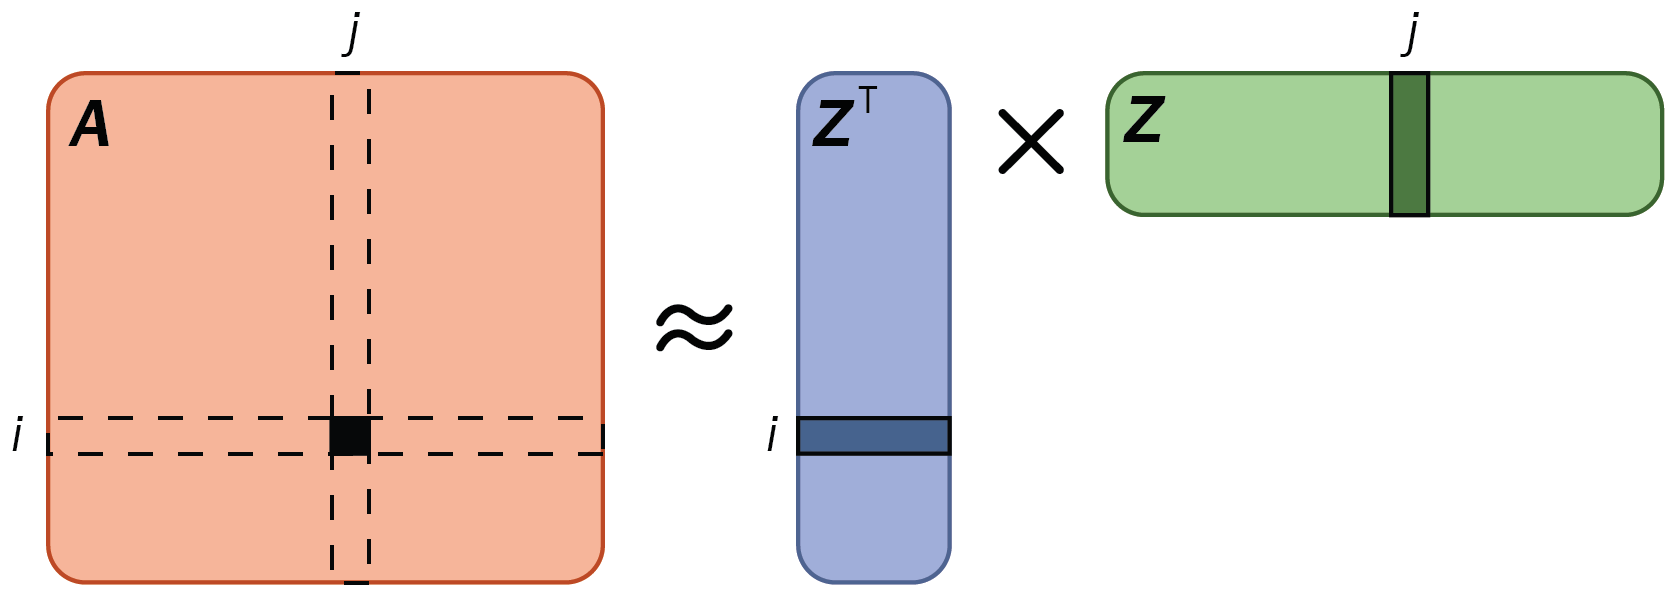
\includegraphics[width=\linewidth]{images/ch10_fig02_gae_decoder_AeqZTZ.png}\\
\tiny (Labonne, 2023)
\end{column}
\end{columns}
\end{frame}

\begin{frame}{GAE의 재구성 손실}
이진 교차엔트로피 형태:
\begin{align*}
  \mathcal{L}_{\text{recon}} =
   - \sum_{(u,v)\in E^{+}} \log \hat{A}_{uv}
   - \sum_{(u,v)\in E^{-}} \log(1-\hat{A}_{uv})
\end{align*}
\begin{itemize}
  \item $E^{+}$: 양성 엣지, $E^{-}$: 무작위 음성 엣지
  \item 클래스 불균형(양성 $\ll$ 음성) 때문에 양/음 같은 수로 샘플링하는 것이 일반적
  \item 단점: 임베딩이 결정적(deterministic) — 노드별 \emph{불확실성}을 표현 못함
\end{itemize}
\end{frame}

% =============================================================
\section{Variational Graph Autoencoder (VGAE)}
% =============================================================

\begin{frame}{VGAE: 확률적 인코더}
각 노드 $i$의 잠재변수 $\mathbf{z}_i$가 가우시안을 따른다고 가정:
\begin{equation*}
  q(\mathbf{z}_i \mid X, A) = \mathcal{N}\bigl(\bm{\mu}_i,\ \mathrm{diag}(\bm{\sigma}_i^2)\bigr)
\end{equation*}
두 개의 GCN으로 평균과 로그분산을 동시에 출력:
\begin{align*}
  \bm{\mu}        &= \mathrm{GCN}_{\mu}(X, A) \\
  \log \bm{\sigma} &= \mathrm{GCN}_{\sigma}(X, A)
\end{align*}
\textbf{재매개화(reparameterization)}: $\mathbf{z} = \bm{\mu} + \bm{\sigma}\odot \bm{\epsilon}$, $\bm{\epsilon}\sim\mathcal{N}(0,I)$
\end{frame}

\begin{frame}{VGAE 손실}
\begin{equation*}
  \mathcal{L}_{\text{VGAE}} = \underbrace{\mathcal{L}_{\text{recon}}}_{\text{엣지 복원}}
    \;+\; \tfrac{1}{N}\;\underbrace{\mathrm{KL}\!\left[q(Z\mid X,A)\,\|\,p(Z)\right]}_{\text{사전분포로의 정규화}}
\end{equation*}
\begin{itemize}
  \item 사전분포 $p(Z) = \mathcal{N}(0,I)$
  \item KL은 정규화 역할 — 임베딩이 너무 자유로워지지 않게 함
  \item 1/N 가중치는 노드 수에 비례한 KL을 노드당 평균으로 정규화하는 효과
  \item 디코더는 GAE와 동일: $\hat{A}_{uv} = \sigma(\mathbf{z}_u^\top \mathbf{z}_v)$
\end{itemize}
\end{frame}

\begin{frame}[fragile]{PyG의 \texttt{VGAE} 인코더 구현}
\begin{lstlisting}
from torch_geometric.nn import GCNConv, VGAE

class Encoder(torch.nn.Module):
    def __init__(self, dim_in, dim_out):
        super().__init__()
        self.conv1       = GCNConv(dim_in, 2 * dim_out)
        self.conv_mu     = GCNConv(2 * dim_out, dim_out)
        self.conv_logstd = GCNConv(2 * dim_out, dim_out)

    def forward(self, x, edge_index):
        x = self.conv1(x, edge_index).relu()
        return (self.conv_mu(x, edge_index),
                self.conv_logstd(x, edge_index))

model = VGAE(Encoder(dataset.num_features, 16)).to(device)
\end{lstlisting}
\begin{itemize}
  \item \texttt{VGAE} 래퍼가 reparameterization, recon\_loss, kl\_loss 제공
\end{itemize}
\end{frame}

\begin{frame}[fragile]{VGAE 학습 루프}
\begin{lstlisting}
def train():
    model.train()
    optimizer.zero_grad()
    z = model.encode(train_data.x, train_data.edge_index)
    loss = model.recon_loss(z, train_data.pos_edge_label_index) \
         + (1 / train_data.num_nodes) * model.kl_loss()
    loss.backward(); optimizer.step()
    return float(loss)

@torch.no_grad()
def test(data):
    model.eval()
    z = model.encode(data.x, data.edge_index)
    return model.test(z, data.pos_edge_label_index,
                         data.neg_edge_label_index)
\end{lstlisting}
\begin{itemize}
  \item \texttt{recon\_loss}는 내부적으로 \emph{음성 엣지를 매 epoch 자동 샘플링}
  \item \texttt{test} 결과: AUC, AP
\end{itemize}
\end{frame}

\begin{frame}{Cora 데이터셋 결과}
\begin{columns}[T,onlytextwidth]
\begin{column}{0.50\textwidth}
\small
\begin{itemize}
  \item Encoder: GCN(1433$\to$32) $\to$ GCN(32$\to$16)$\times 2$
  \item 300 epoch, Adam (lr=0.01)
  \item 책: Test AUC $\approx$ 0.88, AP $\approx$ 0.90
  \item 본 실행(CPU, 시드=0): \textbf{AUC = 0.869, AP = 0.872}
\end{itemize}
\vspace{0.4em}
\footnotesize
$\hat{A}$의 \emph{블록 구조} → 같은 클래스 노드끼리 높은 점수가 매겨짐 (homophily 학습됨).
\end{column}
\begin{column}{0.48\textwidth}
\centering
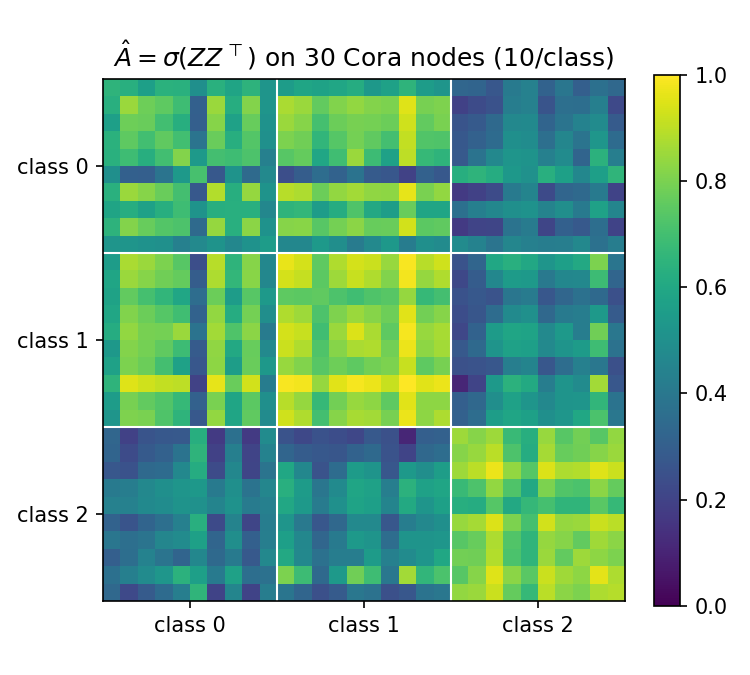
\includegraphics[width=\linewidth]{images/ch10_runtime_vgae_ahat_heatmap.png}
\end{column}
\end{columns}
\end{frame}

\begin{frame}{VGAE 임베딩 시각화 (t-SNE)}
\begin{columns}[c,onlytextwidth]
\begin{column}{0.55\textwidth}
\centering
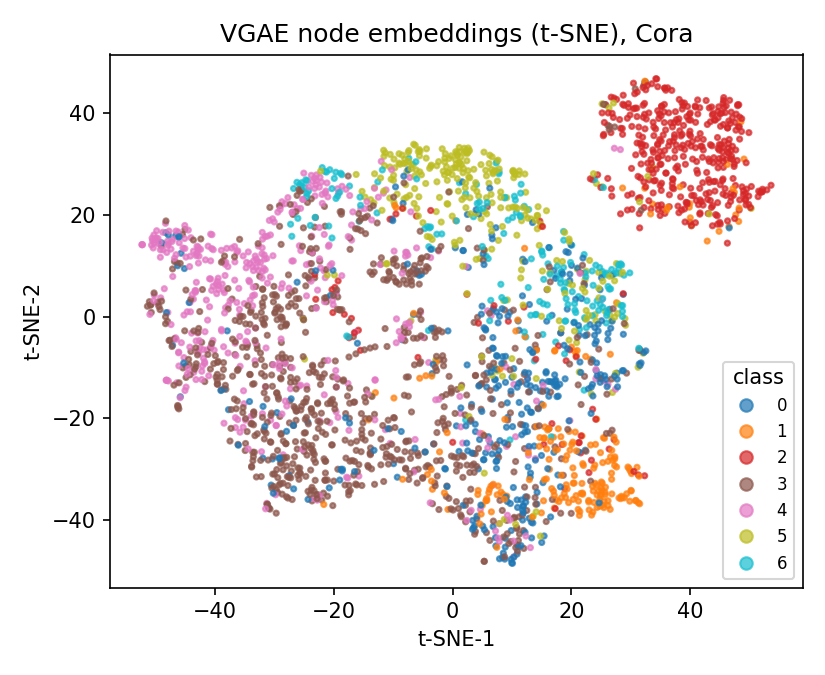
\includegraphics[width=\linewidth]{images/ch10_runtime_vgae_embedding_tsne.png}
\end{column}
\begin{column}{0.42\textwidth}
\small
\begin{itemize}
  \item 16차원 잠재공간 → t-SNE 2D 투영
  \item Cora의 7개 클래스가 \emph{무지도 학습만으로} 어느 정도 군집화됨
  \item 링크 예측만 학습했는데 \textbf{클래스 구조가 자연스럽게 드러남} — homophily 그래프에서 링크와 클래스는 강하게 결합
  \item 단점도 같은 그림에서: 일부 클래스(0, 3)는 임베딩이 흐트러져 있음
\end{itemize}
\end{column}
\end{columns}
\end{frame}

% =============================================================
\section{SEAL: 서브그래프 분류로서의 링크 예측}
% =============================================================

\begin{frame}{SEAL의 출발점}
\centering
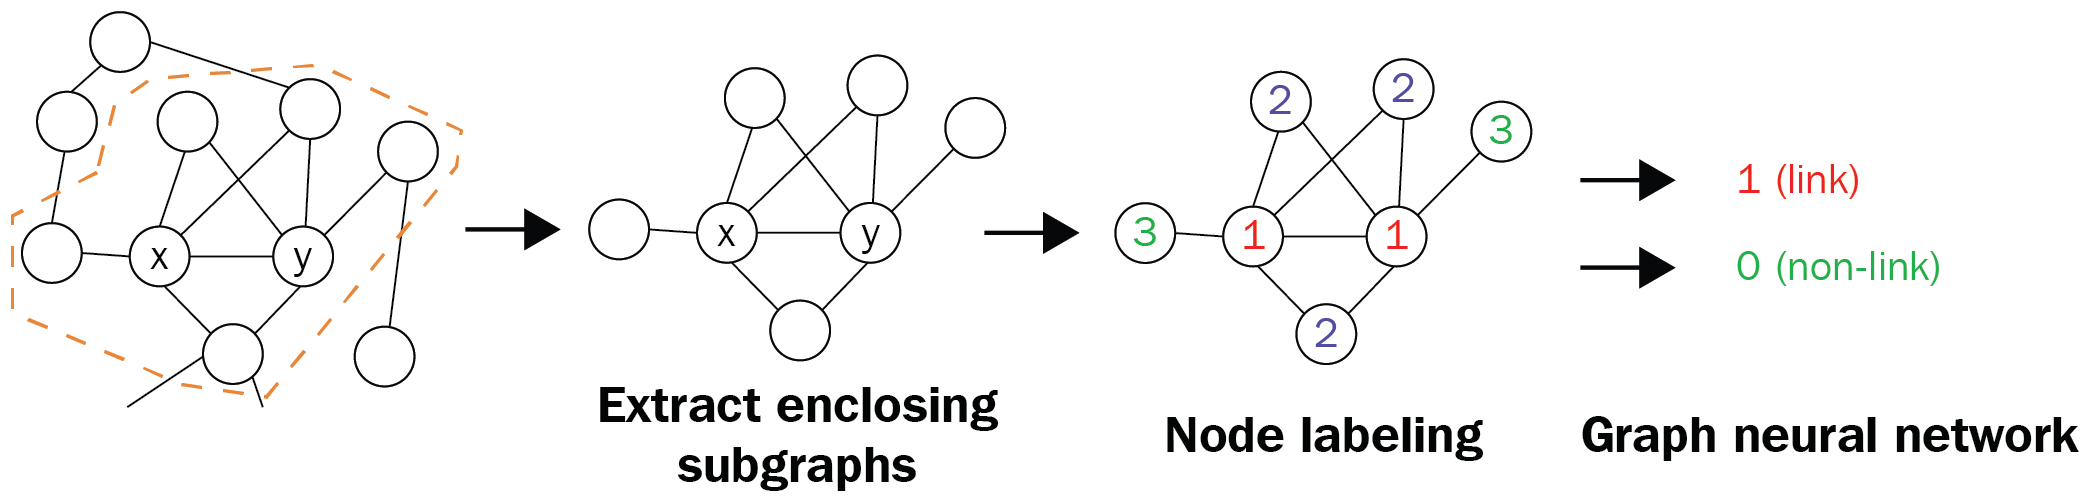
\includegraphics[width=0.95\linewidth]{images/ch10_fig03_seal_pipeline.png}\\
\tiny (Labonne, 2023)
\vspace{0.4em}
\begin{itemize}
  \small
  \item 핵심 통찰: 링크의 존재 여부는 두 노드 \emph{주변의 작은 구조}에 의해 강하게 결정된다.
  \item 휴리스틱(CN, Adamic-Adar, Katz)들이 모두 \textbf{enclosing subgraph}의 함수
  \item 링크 예측을 \textbf{이진 그래프 분류}로 환원: 입력 = 후보 $(u,v)$ 주변 $k$-hop, 출력 = 링크 1/0
\end{itemize}
\end{frame}

\begin{frame}{$k$-hop 이웃 개념}
\begin{columns}[c,onlytextwidth]
\begin{column}{0.52\textwidth}
\centering
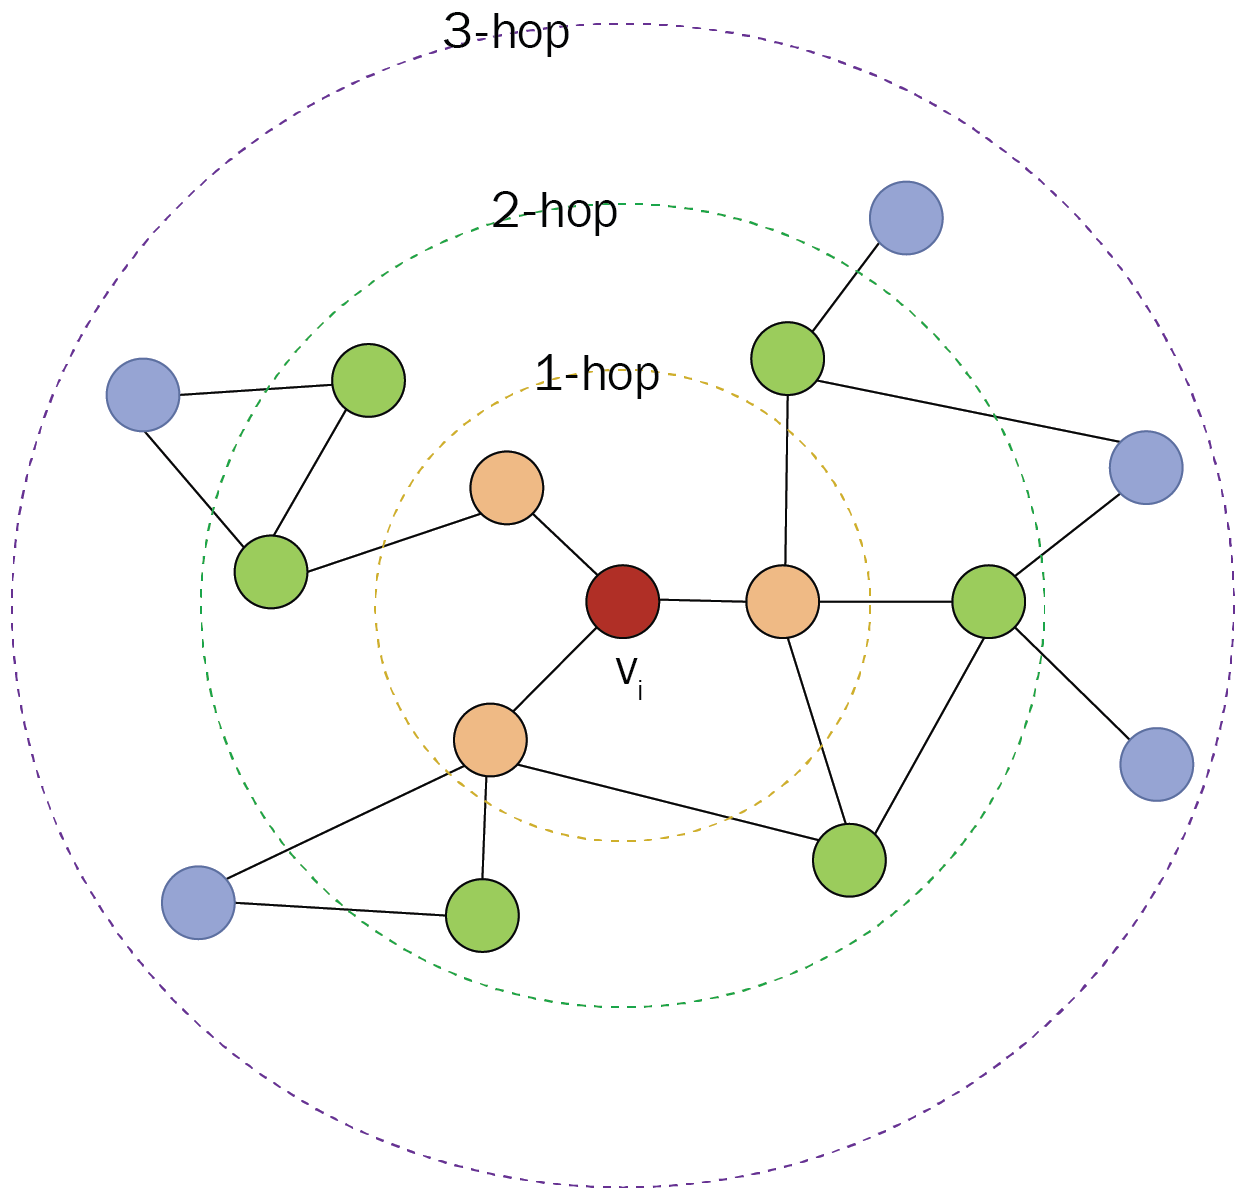
\includegraphics[width=\linewidth]{images/ch10_fig01_khop_neighborhood.png}\\
\tiny (Labonne, 2023)
\end{column}
\begin{column}{0.45\textwidth}
\small
\begin{itemize}
  \item $k$-hop 이웃: 중심 노드로부터 \emph{최대 $k$개의 엣지}로 도달 가능한 노드 집합
  \item SEAL은 \textbf{두 타깃 노드의 $k$-hop 이웃 합집합}을 enclosing subgraph로 사용
  \item $k=2$가 표준 — 너무 크면 비용 폭발, 너무 작으면 정보 부족
\end{itemize}
\end{column}
\end{columns}
\end{frame}

\begin{frame}{Enclosing Subgraph 추출}
\begin{itemize}
  \item 후보 노드 쌍 $(u,v)$에 대해 두 노드의 \textbf{$k$-hop 이웃} 합집합으로 서브그래프 구성
  \item PyG의 \texttt{k\_hop\_subgraph(\{u,v\}, k=2, \ldots, relabel\_nodes=True)}
\end{itemize}
\vspace{0.5em}
\centering
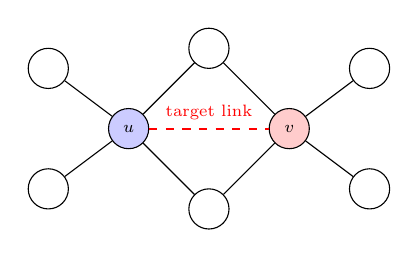
\begin{tikzpicture}[>=Stealth, scale=0.85, every node/.style={transform shape}]
\tikzstyle{n}=[circle,draw,minimum size=6mm,inner sep=0pt,font=\scriptsize]
\node[n,fill=blue!20]  (u) at (-1.2,0)   {$u$};
\node[n,fill=red!20]   (v) at ( 1.2,0)   {$v$};
\node[n] (a) at (-2.4,0.9) {};
\node[n] (b) at (-2.4,-0.9){};
\node[n] (c) at ( 0, 1.2)  {};
\node[n] (d) at ( 0,-1.2)  {};
\node[n] (e) at ( 2.4,0.9) {};
\node[n] (f) at ( 2.4,-0.9){};
\draw (u)--(a); \draw (u)--(b); \draw (u)--(c); \draw (u)--(d);
\draw (v)--(c); \draw (v)--(d); \draw (v)--(e); \draw (v)--(f);
\draw[dashed,red,thick] (u) -- node[above,font=\scriptsize]{target link} (v);
\end{tikzpicture}
\begin{itemize}
  \small
  \item \textbf{타깃 링크 $(u,v)$ 자체는 서브그래프에서 제거} (정답을 보고 학습하면 안 됨)
  \item 학습/평가는 추출된 서브그래프 \emph{전체}의 구조와 노드 정보로 결정
\end{itemize}
\end{frame}

\begin{frame}[fragile]{타깃 엣지 제거 코드}
\begin{lstlisting}
sub_nodes, sub_edge_index, mapping, _ = k_hop_subgraph(
    [src, dst], 2, dataset.edge_index, relabel_nodes=True)
src, dst = mapping.tolist()

# Remove target link from the subgraph
mask1 = (sub_edge_index[0] != src) | (sub_edge_index[1] != dst)
mask2 = (sub_edge_index[0] != dst) | (sub_edge_index[1] != src)
sub_edge_index = sub_edge_index[:, mask1 & mask2]
\end{lstlisting}
\begin{itemize}
  \item 양방향 모두 제거 (\texttt{is\_undirected=True} 가정)
  \item 양성/음성 쌍 모두 동일한 절차로 처리해야 데이터 분포가 일치
\end{itemize}
\end{frame}

\begin{frame}{DRNL: Double-Radius Node Labeling}
타깃 두 노드까지의 거리로 \textbf{각 노드에 라벨}을 부여:
\begin{itemize}
  \item $d_x = d(x,u)$, $d_y = d(x,v)$
  \item 평균 $d=(d_x+d_y)/2$, 모듈로 $r = (d_x+d_y) \bmod 2$
\end{itemize}
\begin{equation*}
  z(x) = 1 + \min(d_x,d_y) + d\cdot(d+r-1)
\end{equation*}
타깃 노드 두 개는 라벨 1 고정, 도달 불가 노드는 0.
\vspace{0.4em}
\textbf{왜 이렇게?}
\begin{itemize}
  \item GNN은 노드 자체에 \emph{누가 타깃인지} 모름 — 라벨로 명시적으로 알려줘야 함
  \item 두 거리를 따로 쓰지 않고 하나의 정수로 인코딩 → one-hot 임베딩이 깔끔
  \item 거리 정보로 휴리스틱(CN, AA, \ldots)의 표현력을 \emph{포함}
\end{itemize}
\end{frame}

\begin{frame}{DRNL 라벨링 예시 (실제 Cora 서브그래프)}
\centering
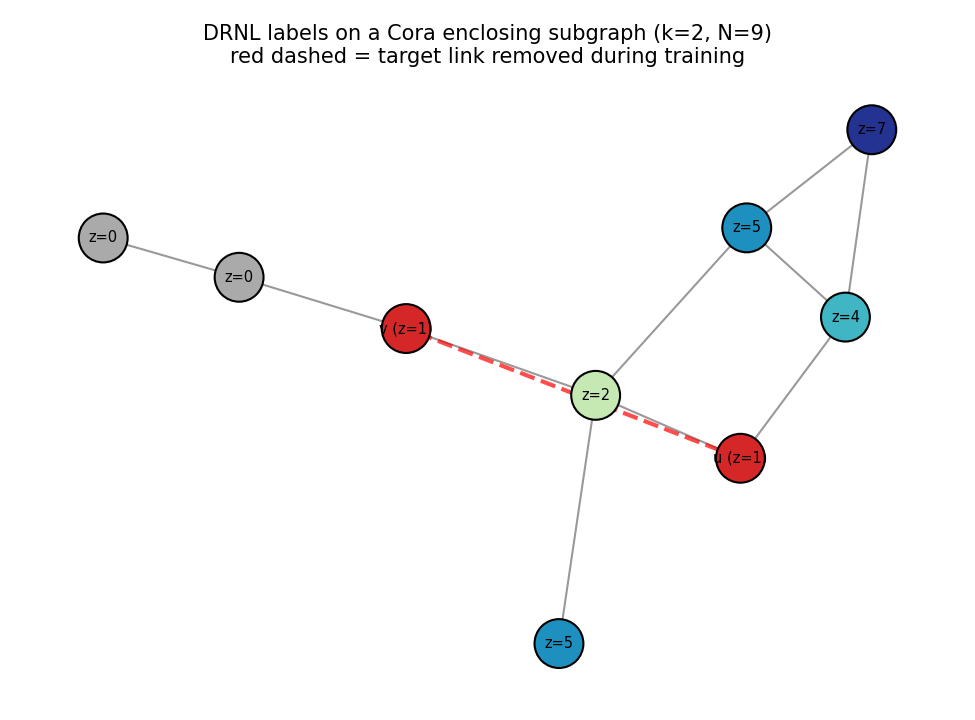
\includegraphics[width=0.85\linewidth]{images/ch10_runtime_drnl_example.png}
\vspace{0.2em}
\footnotesize
\begin{itemize}
  \item 빨간 노드 = 타깃 $(u,v)$, 점선 빨간 엣지 = \emph{제거된} 타깃 엣지
  \item 가운데 $z=2$ 노드는 두 타깃의 공통 이웃 (Common Neighbor) — 휴리스틱이 잡아내는 신호
  \item $z=4,5,7$로 갈수록 타깃에서 먼 노드. $z=0$ 노드들은 src 제거 시 dst 도달 불가
\end{itemize}
\end{frame}

\begin{frame}{SEAL Cora 실행 결과 (본 실행)}
\begin{itemize}
  \item 30 epoch, Adam (lr=$10^{-4}$), BCEWithLogitsLoss
  \item 책 결과: AUC $\approx$ 0.89, AP $\approx$ 0.90
  \item 본 실행(CPU, 시드=0): \textbf{AUC = 0.786, AP = 0.802}
\end{itemize}
\vspace{0.5em}
\textbf{차이 원인 추정}
\begin{itemize}
  \item Epoch 수가 30회로 짧음 — DGCNN은 더 긴 학습에서 안정화됨
  \item BCEWithLogitsLoss를 sigmoid 출력에 사용 (책 코드의 알려진 이슈) — 학습 신호가 약함
  \item 음성 샘플링 매번 무작위라 시드 영향
\end{itemize}
\end{frame}

\begin{frame}[fragile]{DRNL 라벨 계산 (책 코드 발췌)}
\begin{lstlisting}
# d_src : 노드 -> src 거리 (dst를 그래프에서 잠시 제외하고 계산)
# d_dst : 노드 -> dst 거리 (src를 잠시 제외하고 계산)
dist = d_src + d_dst
z = 1 + torch.min(d_src, d_dst) \
      + (dist // 2) * (dist // 2 + (dist % 2) - 1)
z[src], z[dst] = 1., 1.
z[torch.isnan(z)] = 0.

node_labels = F.one_hot(z.to(torch.long), num_classes=200).to(torch.float)
node_emb = node_features  # (선택) 원본 노드 feature 결합
node_x = torch.cat([node_emb, node_labels], dim=1)
data = Data(x=node_x, z=z, edge_index=sub_edge_index, y=y)
\end{lstlisting}
\begin{itemize}
  \small
  \item \texttt{shortest\_path(\ldots, indices=src)}로 거리 계산
  \item \texttt{dst}를 빼고 \texttt{d\_src}를, \texttt{src}를 빼고 \texttt{d\_dst}를 — \emph{경로 누설 방지}
\end{itemize}
\end{frame}

\begin{frame}{DGCNN: SEAL의 분류기}
4-layer GCN → \textbf{SortPooling} → 1D CNN → Dense
\begin{itemize}
  \item \textbf{GCN layers}: 32 → 32 → 32 → 1 채널, \texttt{tanh} 활성, 모두 \emph{concat}
  \item \textbf{SortPooling}: 마지막 채널 기준으로 상위 $k=30$ 노드만 정렬해 고정 길이로
  \item \textbf{Conv1D}: 정렬된 시퀀스를 1D 합성곱으로 처리 → 텍스트 분류 형태
  \item \textbf{Dense $\to$ Sigmoid}: 링크 존재 확률
\end{itemize}
\vspace{0.4em}
서브그래프 크기가 매번 달라도 \emph{고정 차원} 표현을 얻는 것이 SortPooling의 역할.
\end{frame}

\begin{frame}[fragile]{DGCNN 코드 (요지)}
\begin{lstlisting}
class DGCNN(torch.nn.Module):
    def __init__(self, dim_in, k=30):
        super().__init__()
        self.gcn1 = GCNConv(dim_in, 32)
        self.gcn2 = GCNConv(32, 32)
        self.gcn3 = GCNConv(32, 32)
        self.gcn4 = GCNConv(32, 1)
        self.global_pool = aggr.SortAggregation(k=k)
        self.conv1 = Conv1d(1, 16, kernel_size=97, stride=97)
        self.conv2 = Conv1d(16, 32, kernel_size=5, stride=1)
        self.maxpool = MaxPool1d(2, 2)
        self.linear1 = Linear(352, 128); self.dropout = Dropout(0.5)
        self.linear2 = Linear(128, 1)
\end{lstlisting}
\begin{itemize}
  \item GCN 출력을 \emph{layer-wise concat} 한 뒤 SortPool로 $k=30$개 노드 선택
\end{itemize}
\end{frame}

\begin{frame}{트레이드오프}
\textbf{SEAL의 장점}
\begin{itemize}
  \item 표현력이 강함 — DRNL이 거리/구조 정보를 명시적으로 인코딩, 휴리스틱들을 일반화
  \item 인덕티브(inductive): 학습된 모델로 새 그래프에서도 추론 가능
\end{itemize}
\vspace{0.4em}
\textbf{SEAL의 단점}
\begin{itemize}
  \item 후보 링크 하나당 \textbf{서브그래프 추출 + DRNL 전처리}가 필요해 비용이 큼
  \item VGAE는 \emph{한 번의 encode} 후 모든 쌍에 대해 점수를 즉시 계산 가능
  \item 대규모 그래프(수억 노드)에선 사실상 적용 불가
\end{itemize}
\end{frame}

% =============================================================
\section{정리 및 비교}
% =============================================================

\begin{frame}{VGAE vs SEAL 한눈에 보기}
\small
\begin{tabular}{p{0.22\linewidth} p{0.36\linewidth} p{0.36\linewidth}}
\toprule
 & \textbf{VGAE} & \textbf{SEAL} \\
\midrule
관점     & 그래프 전체 임베딩          & 후보 링크별 서브그래프 분류 \\
입력 단위 & 그래프 1개                  & 후보 링크 1개 \\
디코더   & 내적 $\sigma(z_u^\top z_v)$ & DGCNN (GCN+SortPool+Conv1D) \\
노드 라벨 & 원본 feature만             & 원본 feature + DRNL one-hot \\
학습 비용 & 작음                        & 큼 (서브그래프 전처리) \\
추론 비용 & 매우 작음 ($O(d)$/쌍)       & 큼 (쌍마다 서브그래프) \\
표현력   & 대칭/저차원 한계           & 휴리스틱 일반화, 풍부 \\
\bottomrule
\end{tabular}
\end{frame}

\begin{frame}{발제 마무리}
\textbf{핵심 메시지}
\begin{itemize}
  \item 링크 예측은 \emph{쌍에 대한 이진 분류} — 데이터 분할도 \emph{엣지} 단위로
  \item GAE/VGAE: 노드 임베딩 + 내적 디코더, \textbf{확장성}이 강점
  \item SEAL: \emph{서브그래프 분류}로 환원, \textbf{표현력}이 강점
  \item DRNL은 GNN이 ``타깃이 누구인지''를 알게 해주는 명시적 라벨 트릭
\end{itemize}
\vspace{0.5em}
\textbf{다음 장 예고 (Chapter 11): 그래프 생성 모델}
\end{frame}

\begin{frame}{Q\&A}
\centering
\Large 질문 / 토론
\vspace{1em}

\normalsize
\begin{itemize}
  \item VGAE의 KL 항을 $1/N$로 나누는 이유?
  \item SEAL에서 enclosing subgraph의 반경 $k$를 키우면?
  \item 산업 환경(수억 노드)에서 SEAL이 적용 가능할까?
\end{itemize}
\end{frame}

\end{document}
